\chapter{Background}

This chapter describes the theories and knowledge that is used throughout the project. Starting with learning models, with focus on the matrix factorization(MF) method of singular value decomposition(SVD) and variations hereof. Then we describe elements of data preprocessing, testing, and evaluation methods, before the substitute for group decision making by aggregation is described and analyzed. As part of the aggregations we also look at the voting system of single transferable vote(STV).

\section{Learning Model}
Covering some facets of matrix factorization(MF), this section delves into how and why MF can be used as a part of a recommendation system. In specific the methodology of SVD and variations thereof will be explained. 
%\subsection{Classification}

%\subsection{Regression} \label{bg:sub:regression}
Regression is first and foremost known from statistics where Linear Regression uses the basis of designing a prediction function based on a dataset. This function can then be used to predict a value given a variable.
The prediction function generally looks like Equation \ref{eq:regression_general_prediction_function}.

\begin{equation} \label{eq:regression_general_prediction_function}
	Y' = bX + A
\end{equation}

Where \textit{b} is the slope of the function, \textit{A} is the interception with the y-axis, and \textit{Y'} is the predicted score or rating.
To calculate \textit{b} and \textit{A} it is necessary to define several additional values, first and foremost the means of values of \textit{x} and \textit{y} from the dataset. These means are denoted as \textit{$M_{X}$} and \textit{$M_{Y}$} respectively. Then it is possible to calculate the the correlation \textit{r} using Pearson's method seen in Equation \ref{eq:regression_pearsons_correlation}.

\begin{equation} \label{eq:regression_pearsons_correlation}
	r = \frac{\sum x'y'}{\sqrt{\sum x'^{2}\sum y'^{2}}}
\end{equation}

Here \textit{x'} and \textit{y'} are the values of  \textit{x} and \textit{y} minus their respective means \textit{$M_{X}$} and \textit{$M_{Y}$}. Now \textit{r} can be used in Equation \ref{eq:regression_slope_calculation} to get \textit{b}.

\begin{equation} \label{eq:regression_slope_calculation}
	b = r\frac{S_{Y}}{S_{X}}
\end{equation}

Here there is still a need to calculate \textit{$S_{X}$} and \textit{$S_{Y}$} that are the standard deviations for \textit{x} and \textit{y} respectively. However this is trivial. When \textit{b} has been computed it can be used to finally calculate \textit{A} using Equation \ref{eq:regression_intersection_calculation}.

\begin{equation} \label{eq:regression_intersection_calculation}
	A = M_{Y} - bM_{X}
\end{equation}

As Linear Regression showcases, the principle in regression is to construct a function, based on a dataset, used to predict the value of \textit{Y} based on the value \textit{X}. However, while this is useful when only one variable is taken into account, it becomes increasingly ill-suited when the number of comparable variables expand.
\subsection{Matrix Factorization Models} \label{bg:sub:factorizationmodels}
%Function
Matrix Factorization Model methods are dimensionality reduction techniques used for recommendation that generally find latent features for items, and the propensity for users towards each latent feature.
Matrix Factorization (MF) makes an approximation of a matrix of ratings by decomposing it into multiple matrices. Since MF approximates matrices in an offline step before recommendation, it scales better compared to contemporary Collective Filtering techniques during recommendation. It performs well even when data sparsity is a concern due to the matrix approximation and the dimensionality reduction.
As data sparsity grows in a set, the less accurate every method gets. Factorization methods counteract this by compressing the data, making it less sparse, and easier to cluster.
As an MF matrix is traditionally updated offline resulting in unchanging matrices, then the matrix can be reused as required. This is a benefit when testing various aggregations or configurations of users.

\subsubsection{Singular Value Decomposition}
Commonly referred to by its acronym, SVD, was popular during Netflix's movie recommender contest amongst the top performing entrants.

On its own, SVD is a dimensionality reduction technique. However in 2006 Simon Funk \cite{svdsimonfunk} popularized it as a recommender method with some modifications.

Given a matrix of user ratings, SVD works by decomposing the matrix as seen in equation \ref{eq:svd_decomp} into two matrices called the left and right singular vectors, $U$ and $V$ respectively, and a matrix holding the singular values on its diagonal, $\Sigma$, as per the SVD theorem\cite{svdtheorem}. For this example, the left singular vector would hold the users on one side, and their inclination towards each latent feature. The right vector would conversely hold all the rated items, and their inclination towards each latent feature.

\begin{equation} \label{eq:svd_decomp}
\centering
M = U\times \Sigma \times V^T
\end{equation}

SVD considers as many features as there are ranks, but not all of them are influential. Reducing the number of features to consider is trivial, as the largest singular values stored in $\Sigma$ have the most influence.

At this point, it is possible to find some interesting similarities among the users, however to use SVD for recommendation, we must account for the missing ratings. By slightly tweaking the equation, as seen in \ref{eq:svd_AB_squeezing}, we get an A and B matrix, holding users and items respectively. This is results in three matrices looking like \ref{fig:svd_squeeze}\todo{Fix ref to figure below}.

\begin{equation}\label{eq:svd_AB_squeezing}
	\centering
	U\times \Sigma \times V^T = U\Sigma^{1/2} \Sigma^{1/2}V^T = AB
\end{equation}

\begin{figure} [H] \label{fig:svd_squeeze}
	\centering
	\includegraphics[scale=0.75]{svd_ab_squeeze.png}
	\caption{The decomposition of a rating matrix using SVD}
\end{figure}
\todo{Temporary figure from course slides - replace with own}

Having moved to the dense subspace of each rated item and user being defined by their features rather than their explicit ratings, data sparsity becomes less of a problem, as missing ratings are squeezed out.

\subsubsection{Gradient descent}
In Funk's blog, the gradient descent optimization algorithm is proposed as a common method to learn the A and B matrices to minimize the error, as found using Equation \ref{eq:gradient_descent_error}. The error is calculated as the euclidean distance between our known ratings, $R$, and our predicted ratings $\hat{R}$.

\begin{equation}\label{eq:gradient_descent_error}
\text{Error} = |R-\hat{R}| = |R - AB| = \sum_{u=1}^{U}\sum_{i=1}^{I}\left (R_{ui}- \sum_{k=1}^{K} A_{uk}B_{ki} \right )^2
\end{equation}

Given as a function, the gradient will point in the direction of the largest error increase, as shown in equation \ref{eq:derivative_gradient}. So to minimize the error, steps are taken towards the negative of the gradient.

\begin{equation}\label{eq:derivative_gradient}
	\begin{split}
	\frac{dError}{dA}=-(R-AB)B^T = \sum_{i=1}^{I}(R_{ui} - \sum_{n=1}^{N} A_{un}B_{ni})B_{ki}
	\\
	\frac{dError}{dB}=-(R-AB)A^T = \sum_{u=1}^{U}(R_{ui} - \sum_{n=1}^{N} A_{un}B_{ni})A_{uk}
	\end{split}
\end{equation}

Taking the average error when finding the derivative is a costly operation for learning the A and B matrices, as it sums up the error for every user-item pair across all of their features. This can be expressed by a running time as shown in equation \ref{eq:gradient_descent_runningtime}.

\begin{equation}\label{eq:gradient_descent_runningtime}
	\Theta(U\times I \times K)
\end{equation}

The common solution is using the stochastic gradient descent. For this, a single observed rating is selected at random for each update step of the gradient descent, rather than summing up over all the item-user pairs to find the exact gradient. The updates will be a bit more erratic, but will overall tend towards the gradient, as seen in figure \ref{fig:gradient_descent}.

\begin{figure}\label{fig:gradient_descent}
	\centering
	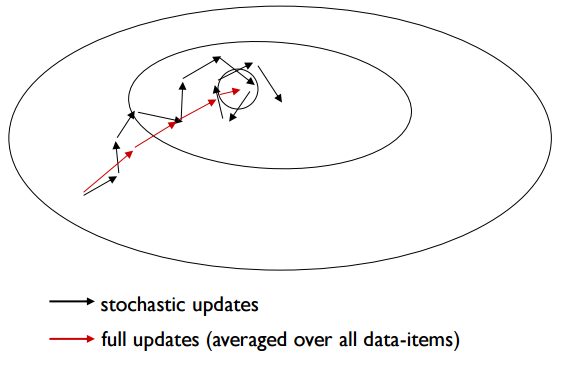
\includegraphics[scale=0.5]{gradient_descent.png}
	\caption{Gradient descent comparison with the stochastic variant as they mvoe towards the gradient}
\end{figure}

\todo{Describe regularization used}


\subsubsection{Non-negative Matrix Factorization}

Non-negative Matrix factorization is a constraint on the usual matrix factorization. All values are equal to 0 or higher, and always positive, and when learning the model, no values will dip below 0.

As shown in \ref{eq:nmf}, given a rating matrix of size \textit{m-by-n}, for example m users and n items, we can find non-negative matrix factors $W$ and $H$ of size \textit{m-by-k} and \textit{k-by-n} such that they approximate $V$.

\begin{equation} \label{eq:nmf}
	V \approx W H
\end{equation}

%http://www.kyb.mpg.de/fileadmin/user_upload/files/publications/attachments/CFEMF_KDDW2007_4614[0].pdf
\subsubsection{SVD++} \label{bg:mf_svd++}
As the name implies, SVD++ is an extension on SVD. Where SVD in general only works with explicit data, SVD++ takes into account the implicitly gathered data as well. Take for instance a user that have a number of items they have shown some indirect interest in, for instance hovering over the items to see some information about them, SVD++ would specifically account for this set of potentially interesting items. All the information in this section has been gathered from "Recommender Systems Handbook" \cite{recsyshandbook}.


\note{Move this part about standard SVD to the appropriate section in the report along with the equation for it.} \todo{Make sure the notation and explanations are correct.}
The standard model for SVD can be seen in Equation \ref{eq:svd_standard}, where $\hat{r}_{ui}$ is the predicted rating, $\mu$ is the overall average rating, $b_{i}$ and $b_{u}$ are the deviations from the average for item $i$ and user $u$ respectively, and $q_{i}^{T}p_{u}$ is a representation of the interaction between user $u$ and item $i$, in other words the overall interest in aspects of the item from the user.

\begin{equation} \label{eq:svd_standard}
\centering
\hat{r}_{ui} = \mu + b_{i} + b_{u} + q_{i}^{T}p_{u}
\end{equation}

In SVD++ the last part of the model is altered, to reflect how users are characterized based on the items they have rated, as seen in Equation \ref{eq:svd++_standard}. Here $R(u)$ is the set of items rated by the user $u$, and $y_{j}$ is a factor vector. $p_{u}$ is a free user-factors vector.

\begin{equation} \label{eq:svd++_standard}
\centering
\hat{r}_{ui} = \mu + b_{i} + b_{u} + q_{i}^{T}\left (p_{u} + \left | R(u) \right |^{-\frac{1}{2}} \sum_{j\in R(u)} y_{j} \right )
\end{equation}

There is in theory no limit to the number of itemsets that can be inferred and accounted for, each would simply have its own item factor vector, as seen in Equation \ref{eq:svd++_multi}.

\begin{equation} \label{eq:svd++_multi}
\centering
\hat{r}_{ui} = \mu + b_{i} + b_{u} + q_{i}^{T}\left (p_{u} + \left | N^{1}(u) \right |^{-\frac{1}{2}} \sum_{j\in N^{1}(u)} y_{j}^{(1)} + \left | N^{2}(u) \right |^{-\frac{1}{2}} \sum_{j\in N^{2}(u)} y_{j}^{(2)} \right )
\end{equation}

SVD++ in general performs better than SVD, however if there is no implicit data, the uses for SVD++ becomes negligible.

\subsubsection{Choice of Recommender system}\label{sec:decision} %if label is changed then also change it in Individual recommendation.
For this problem, we went with the matrix factorization. Matrix factorization wins out in general since the offline training makes us able to reuse a model once it has been trained for the multiple tests. SVD also has several other notable benefits, such as finding otherwise hidden correlations in the data.

Among the different matrix factorization approaches, we went with the standard SVD, as the SVD++ method is better suited for data with implicit connections.
\subsubsection{Non-negative Matrix Factorization}

NMF is a constraint on the standard MF. All values are equal to or higher than 0, and when learning the model, no values can go below 0, which is ensured by setting any values that have become negative back to 0 before the next iteration. This is helpful for speeding up the learning in certain domains, for instance finding objects or parts hereof in images\cite{nnmf}.

As shown in Equation \ref{eq:nmf}, given a rating matrix of size \textit{m-by-n}, for example m users and n items, we can find non-negative matrix factors $W$ and $H$ of size \textit{m-by-f} and \textit{f-by-n} respectively, such that they approximate $V$. During this $f$ is usually chosen to be smaller than the rank of the $m$ by $n$ matrix, as to reduce the size of $W$ and $H$ compared to the original matrix, $V$\cite{LeeNMF}.

\begin{equation} \label{eq:nmf}
	V \approx W H
\end{equation}

%Furthermore, a property of NMF is that it can be rewritten as seen in Equation \ref{eq:nnmf_rewritten}, where $i$ is the index of the columns in $V$ and $H$. This means that the data vector $v_{i}$ is an approximation given by a linear combination of the columns of $W$, weighted by $h_{i}$ components\cite{LeeNMF}.

%\begin{equation} \label{eq:nnmf_rewritten}
%	v_{i} \approx W h_{i}
%\end{equation}

As an example of NMF, if we consider the $A$ and $B$ matrices found in Equation \ref{eq:svd_AB_num_squeezing} to be our potential $W$ and $H$ matrices without the constraint, we would with NMF get a result as in Equation \ref{eq:nmf_example}.

\begin{equation}\label{eq:nmf_example}
\begin{split}
W =
\begin{bmatrix}
0 & 0.13 & 0\\
0 & 0 & 0.14\\
0 & 0.9 & 0.3
\end{bmatrix}
\\
H = 
\begin{bmatrix}
0 & 0 & 0\\
1.15 & 0 & 0\\
0.45 & 0.54 & 0
\end{bmatrix}
\end{split}
\end{equation}
\subsubsection{Choice of Recommender system}\label{sec:decision} %if label is changed then also change it in Individual recommendation.
For this problem, we went with matrix factorization. Matrix factorization wins out in general since the offline training makes us able to reuse a model once it has been trained for the multiple tests. SVD also has several other notable benefits, such as finding otherwise hidden correlations in the data.

Among the different matrix factorization approaches, we went with the standard SVD, because SVD is a standard method, so it is more easily replicated by other studies and there are many libraries available for it. The precision of the recommender is also not the main focus of this project, as the satisfaction of the group is not improved by a better precision.
\section{Data Processing}\label{sec:data_preprocessing}
For this project we are using the Movielens 100k data set which contains 100000 ratings, between 1 and 5, from 943 user spread out on 1682 movies\cite{movielens100k}. 

Notes:
The data set was separated into 5 folds
\subsection{Preprocessing}
In order to use the data set for matrix factorization we need to present it in a matrix. 

Notes: 
Extract different users and movies.
Constructing matrices of the folds and the total data set.
Making new base folds containing all items 


\section{Testing and Evaluation}
This section covers the testing and evaluation methods we will use. In specific k-fold testing and our evaluation metrics will be explained.

\subsection{K-fold Testing}
Stemming from cross validation in the field of statistics, k-fold testing is a commonly used technique in regards to recommender systems\cite{kfold}. The basic principle in the method is to split the dataset into $k$ equally sized parts or folds, and then use one of the folds as the testing or validation set, while the rest of the folds are used as training data. This process is then repeated $k$ times, so each fold is used as the validation set once. After it has been repeated $k$ times, the results can then be averaged to find an overall estimation of the error in the model. An example of how the k-fold ordering could be structured can be seen in Table \ref{tbl:bg_k-fold}. Typically, either 5-fold or 10-fold testing is what is used.

\begin{table}[H]
	\centering
	\begin{tabular}{|l|c|c|c|c|}
		\hline
		& \multicolumn{3}{l|}{Training} & \multicolumn{1}{l|}{Validation} \\ \hline
		First  & 1        & 2        & 3       & 4                               \\ \hline
		Second & 2        & 3        & 4       & 1                               \\ \hline
		Third  & 3        & 4        & 1       & 2                               \\ \hline
		Forth  & 4        & 1        & 2       & 3                               \\ \hline
	\end{tabular}
	\caption{Example of the rotation of folds in a 4-fold dataset}
	\label{tbl:bg_k-fold}
\end{table}

\subsection{Evaluation Metrics}
Here we will cover the various evaluation metrics used in the project. MAE and RMSE are considered for the recommender for tuning, and nDCG is presented for evaluating satisfaction with a recommendation.

\subsubsection{Root Mean Square Error}
The root mean square error(RMSE) is a common accuracy measure for recommender systems\cite{rmse}. For the algorithm, RMSE is calculated using the Equation \ref{eq:background_rmse}. $\tau$ is the set of user item pairs used to validate the system, with $u$ and $i$ being user and item, respectively. $\hat{r}_{ui}$ are the predicted ratings for a user item pair, from which we subtract the actual rating, $r_{ui}$, to find the error.

\begin{equation} \label{eq:background_rmse}
\text{RMSE} = \sqrt{\frac{1}{|\tau|}\sum_{(u,i)\in \tau}(\hat{r}_{ui}-r_{ui})^2}
\end{equation}

An alternative, mean absolute error(MAE), as seen in Equation \ref{eq:background_mae}, takes the euclidean distance rather than the squared difference\cite{rmse}. As opposed to MAE, RMSE penalizes larger errors relatively more harshly.

\begin{equation} \label{eq:background_mae}
\text{MAE} = \frac{1}{|\tau|}\sum_{(u,i)\in \tau}|\hat{r}_{ui}-r_{ui}|
\end{equation}

For this project, we used RMSE in the evaluation of the SVD module of the recommender system. On this system, the RMSE equation is amended to the form shown Equation \ref{eq:background_svd_rmse}, where $U$ is a set of users, $I$ is a set of items, and $F$ is a set of features. $R$ is the rating matrix.

\begin{equation}\label{eq:background_svd_rmse}
	\text{RMSE} = \sqrt{\frac{\sum_{u=1}^{U}\sum_{i=1}^{I}(\sum_{f=1}^{F}(A_{uf} B_{fi}) - R_{ui})^2}{|U|\times |I|\times |F|}}
\end{equation}

\subsubsection{Normalized Discounted Cumulative Gain}\label{sec:testandeval_ndcg}
Discounted cumulative gain is used to measure the quality of a ranking through the relevance of the result set. It is most commonly used in the information retrieval field for determining the quality of the result of a query, however it is also useful for getting a measure of satisfaction for an ordering of recommended items. That is because recommendation and the results of a search query are both solutions to the problem of information overload that presents a set of possible items\cite{ndcg}\cite{baltrunas}.

For a group recommendation this works by comparing the group recommendation with the individual preferences. In this way, the relevance of an item is translatable to a ranked list of recommendations, as a recommendation can be viewed as a fixed query.

The measure grew out from the Cumulative Gain measure, which takes the relevance score of each result in a set without considering the position in the set. Equation \ref{eq:background_cg} shows the process. $p$ denotes the number of positions in the ranking.

\begin{equation}\label{eq:background_cg}
	\text{CG}_p = \sum_{i=1}^{p}\textit{rel}_i
\end{equation}

The addition of the discounted property adds a consideration over the ranking. For most lists, it is assumed that a user will consider each item in order from first to last, making the most important position the first item. So it follows that the most relevant item should be the first item. This justifies penalizing a deviance from ordering by the most relevant item first. The score is calculated using Equation \ref{eq:background_dcg}.

\begin{equation}\label{eq:background_dcg}
	\text{DCG}_p = \sum_{i=1}^{p}\frac{\textit{rel}_i}{\log_2(i + 1)}
\end{equation}

Normalized discounted cumulative gain compares the DCG with an ideal ranking as to normalize the score, where a perfect ordering results in a score of 1, so it can be compared for systems using rankings of different lengths. The score is calculated using Equation \ref{eq:background_ndcg}. The IDCG is the ideal DCG with basically is the elements in DCG sorted in the order of relevance.

%The ideal ranking is IDCG, which is calculated using Equation \ref{eq:background_idcg}, where we use the individual's list of preferences as the basis for an ideal ranking for that user.

\begin{equation}\label{eq:background_ndcg}
	\text{nDCG}_p = \frac{\text{DCG}_p}{\text{IDCG}_p}
\end{equation}

%\begin{equation}\label{eq:background_idcg}
%	\text{IDCG}_p = \sum_{i=1}^{|REL|} \frac{2^{\textit{rel}_i}-1}{\log_2(i+1)}
%\end{equation}

As an example of finding the satisfaction of a user based on the recommendations for the group, the rating of a group of users can be as seen in Table \ref{tbl:testandeval_bordacount}. User U1 will be the focus of this example, and in Table \ref{tbl:testandeval_positions}, the groups 4 most preferred items, based on average, is shown together with user U1's 4 most preferred items. As can be seen item M8 and M4 overlaps for the two lists giving us a relevance scores for U1 on 9, 9, 0, 0. The two last relevance scores are zero because they are not present in U1's top 4 preferences which we look at in this case.

\begin{table}[H]
	\centering
	\begin{tabular}{l|l|l|l|l|l|l|l|l|l|l|}
		\cline{2-11}
		& M1 & M2 & M3 & M4 & M5 & M6 & M7 & M8 & M9 & M10 \\ \hline
		\multicolumn{1}{|l|}{U1} & 2 & 4 & 5 & 9 & 1 & 3 & 7 & 9 & 8 & 6 \\ \hline
		\multicolumn{1}{|l|}{U2} & 5 & 8 & 9 & 4 & 3 & 6 & 2 & 10 & 1 & 7 \\ \hline
		\multicolumn{1}{|l|}{U3} & 4 & 6 & 2 & 7 & 8 & 3 & 1 & 4 & 10 & 9 \\ \hline
		\multicolumn{1}{|l|}{U4} & 10 & 8 & 2 & 7 & 1 & 4 & 6 & 5 & 8 & 3 \\ \hline
		\multicolumn{1}{|l|}{U5} & 1 & 5 & 9 & 5 & 4 & 2 & 8 & 10 & 2 & 7 \\ \hline
		\multicolumn{1}{|l|}{Total} & 22 & 31 & 27 & 32 & 17 & 18 & 24 & 38 & 29 & 32 \\ \hline
	\end{tabular}
	\caption{Example of ratings for a set of items}
	\label{tbl:testandeval_bordacount}
\end{table}

\begin{table}[H]
	\centering
	\begin{tabular}{l|l|l|l|l|}
		\cline{2-5}
		& I1 & I2 & I3 & I4\\ \hline
		\multicolumn{1}{|l|}{Group ranking} & M8 & M4 & M10 & M2\\ \hline
		\multicolumn{1}{|l|}{U1 ranking} & M8 & M4 & M9 & M7\\ \hline
	\end{tabular}
	\caption{Indices of the group preferences and user U1}
	\label{tbl:testandeval_positions}
\end{table}

The cumulative gain of the example results in a high count in Equation \ref{eq:background_cg_example}, as to be expected as the group and U1 share many preferences in the list. When we consider the positioning in Equation \ref{eq:background_dcg_example}, there is only a small drop in the score, as the bulk of U1's points are at the top positions where the penalty is smaller.

\begin{equation}\label{eq:background_cg_example}
\text{CG}_4 = \sum_{i=1}^{4}\textit{rel}_i = 9 + 9 + 0 + 0 = 18
\end{equation}

\begin{equation}\label{eq:background_dcg_example}
\text{DCG}_4 = \sum_{i=1}^{4}\frac{\textit{rel}_i}{\log_2(i + 1)}
= 9 + 5.68 + 0 + 0 = 14.68
\end{equation}

To normalize the score, we compare it to the ideal ranking, which is U1's own ranking which would be 9, 9, 8, 7. The score for the ideal ordering is calculated in Equation \ref{eq:background_idcg_example}. The level of satisfaction for U1 for this recommendation is $0.68$ equal to a 68\% points, as per Equation \ref{eq:background_ndcg_example}. 

\begin{equation}\label{eq:background_idcg_example}
\text{IDCG}_4 = 9 + 5.68 + 4 + 3.05 = 21.73
\end{equation}

\begin{equation}\label{eq:background_ndcg_example}
\text{nDCG}_4 = \frac{\text{DCG}_4}{\text{IDCG}_4} = \frac{14.68}{21.73}=0.68
\end{equation}

This is an above average score, because even though only 50\% of U1's list is represented, it is the highest ranked items and they are highly ranked on the groups list which is why the percentage point is 68\% and not 50\%. 

\section{Aggregation} \label{bg:aggregation}
When working with a group recommender system, it is hard to avoid using aggregation to make group-like decisions. While recent research has shown that aggregation is not a perfect substitute for group based decisions \todo{insert cite}, it is not our goal to find a suitable substitution for aggregation. We will instead use existing aggregation strategies to find suitable recommendations for the group. While specific strategies are as numerous as the number of recommenders, they are derived from only a few common strategies. Most of these strategies will here be presented using the ratings in Table \ref{aggregation:tbl:table_of_ratings}, while the full overview of the results of aggregation can be seen in Table \ref{aggregation:tbl:examples_of_strategies}.

%\begin{itemize}
%	\item Plurality Voting
%	\item Average
%	\item Multiplicative
%	\item Approval Voting
%	\item Least Misery
%	\item Most Pleasure
%	\item Average Without Misery
%	\item Fairness
%	\item Dictatorship
%\end{itemize}

\begin{table}[H]
	\centering
	\begin{tabular}{ | p{2cm} | p{1cm} | p{1cm} | p{1cm} | p{1cm} | p{1cm} | p{1cm} | p{1cm} | } \hline
		 & \textbf{A} & \textbf{B} & \textbf{E} & \textbf{D} & \textbf{E} & \textbf{F} & \textbf{G}  \\ \hline
		John & 9 & 4 & 7 & 10 & 5 & 1 & 2 \\ \hline
		Jane & 10 & 10 & 5 & 1 & 8 & 7 & 4 \\ \hline
		Bob & 1 & 8 & 4 & 4 & 6 & 10 & 6 \\ \hline
		Hilda & 1 & 7 & 2 & 9 & 5 & 10 & 3 \\ \hline
	\end{tabular}
	\caption{Arbitrary examples of ratings given by four people. The ratings were chosen to showcase the differences in the aggregation strategies.}
	\label{aggregation:tbl:table_of_ratings}
\end{table}

\textbf{Plurality Voting} attempts to gain satisfaction by selecting the items with the highest ratings for the majority of the group first, and then repeating this strategy removing any items already selected. Outlier cases can result in a minority of highly dissatisfied users, simply because their ratings are insignificant. For instance items A being rather highly scored despite two people hating it.\\

\textbf{Average} is one of the simplest ways of aggregating, by simply taking the average of the ratings for an item. As with any averaging, this is not necessarily the best approach as low ratings can be overshadowed by a significantly higher amount of high ratings. This is for instance the case with item F, where the low rating from John is overlooked in favor of the other people's ratings.\\

\textbf{Multiplicative} attempts to improve satisfaction by multiplying each rating for an item with each other, so outlier ratings at either end of the rating scale becomes more significant. This is especially true for the lowest rating, commonly adjusted to be 1, as the rating adds nothing to combined rating. Thereby items receiving the lowest rating by even a small amount of group members quickly fall towards the bottom of the recommendation. For instance this is seen in item D, where Jane's low rating drags the overall score down.\\

\textbf{Approval Voting} transforms the ratings into points for each item. The points are awarded for each group member who have a rating for the item above a certain threshold. In small groups the strategy leads to many ties, in larger groups these ties become more uncommon. In the example item E is approved by every member, and with the threshold set at 5 this is an indication that no member would be dissatisfied with this item.\\

\textbf{Least Misery} attempts to reduce the amount of misery felt by the group by using the lowest rating for an item. This leaves the items to be easily be sorted by how well they are liked by the person who likes them the least. However it also has outlier cases with items well liked by the vast majority but disliked by a single person leaving it with a low rating. This is clearly seen in item F, where John's low rating makes the item seem irrelevant despite it being highly regarded by the other three.\\

\textbf{Most Pleasure} attempts to maximize the satisfaction of the group by only using the highest rating for an item. Like the Least Misery strategy, this suffers from outlier cases going in the other direction, a single person rating an item disliked by the vast majority leaves the item with a high rating. This can be seen in item A, where it ends up with a tie for best choice, despite being hated by half the group members.\\

\textbf{Average Without Misery} works on the concept of removing as much misery as possible, this strategy removes items who have any ratings below a certain threshold, before averaging the ratings of the remaining items. However Average Without Misery suffers from outlier cases just as much as Least Misery and Most Pleasure. The example showcases another problem, where even if one person has given a rating below the threshold, then the item is completely disregarded, therefore this strategy is unsuitable at even small group sizes. In the example only two out of seven items are left for consideration.\\

\textbf{Fairness} goes by the principle of everyone-gets-a-choice, is the essence of Fairness. The items are selected in turn by each group member, and in the purest form the selection is based purely on that member's terms without regarding ratings from others. However ratings from other group members are typically used in case the selecting member has a tie between two or more items. In the example the pure form is used and notable items include item E, which has fairly high ratings from everyone but not the highest rating from anyone, leaving it to be selected second to last.\\

\textbf{Dictatorship} is also called Most Respected Decides. Letting one person and their ratings decide everything is an approach often used in real world scenarios, for instance music being decided by a dj or the movie to watch being decided by the host. However deciding which person to use as the “dictator” is typically handled using trust or respect, hence the alternative name for the strategy. Trust is difficult to measure, especially the more randomly put together the group is.

\begin{table}[H]
	\centering
	\begin{tabular}{ | p{2.5cm} | p{1cm} | p{1cm} | p{1cm} | p{1cm} | p{1cm} | p{1cm} | p{1cm} | } \hline
		& \textbf{A} & \textbf{B} & \textbf{E} & \textbf{D} & \textbf{E} & \textbf{F} & \textbf{G}  \\ \hline
		Plurality Voting & 5 & 4 & 2 & 6 & 3 & 7 & 1 \\ \hline
		Average & 5.25 & 7.25 & 4.5 & 6 & 6 & 7 & 3.75 \\ \hline
		Multiplicative & 90 & 2240 & 280 & 360 & 1200 & 700 & 144 \\ \hline
		Approval Voting (Threshold 5) & 2 & 3 & 2 & 2 & 4 & 3 & 1 \\ \hline
		Least Misery & 1 & 4 & 2 & 1 & 5 & 1 & 2 \\ \hline
		Most Pleasure & 10 & 10 & 7 & 10 & 8 & 10 & 6 \\ \hline
		Average Without Misery (Threshold 4) & - & 7.25 & - & - & 6 & - & - \\ \hline
		Fairness (Start at John) & 6 & 4 & 3 & 7 & 2 & 5 & 1 \\ \hline
		Dictatorship (Hilda) & 1 & 7 & 2 & 9 & 5 & 10 & 3 \\ \hline
	\end{tabular}
	\caption{Examples of the scores that results from applying the individual aggregation strategies to the ratings from Table \ref{aggregation:tbl:table_of_ratings}. All values have been adjusted so the highest value is the 'best'.}
	\label{aggregation:tbl:examples_of_strategies}
\end{table}

\subsection{Simulating Group Behavior}
In the study conducted by Judith Masthoff, it was found that some of the aggregation strategies were used when a group made decisions on which items to recommend, while other strategies provided better recommendations according to the groups. The strategies groups seemed to make use of were, Average, Average Without Misery, and Least Misery. In contrast to this strategies such as Multiplicative, Average, and Most Pleasure gave reasonable recommendations, showing some mismatch between what the group would recommend themselves, and what they retroactively think is best.

However these strategies were looked at independently. By combining different strategies, not only does it reduce or remove some of the downsides to using a specific strategy, it can also improve the recommendations and the satisfaction they lead to.